% Template for IGARSS-2018 paper; to be used with:
%          spconf.sty  - LaTeX style file, and
%          IEEEbib.bst - IEEE bibliography style file.
% --------------------------------------------------------------------------
\documentclass{article}
\usepackage{spconf,amsmath,epsfig,graphicx}
\usepackage{subcaption}

% Example definitions.
% --------------------
\def\x{{\mathbf x}}
\def\L{{\cal L}}

% Title.
% ------
\title{Unsupervised Sequential Classification of MODIS Time-Series}
%
% Single address.
% ---------------
\name{T.L. Grobler$^{\dagger}$, W. Kleynhans$^{\star}$ and B.P. Salmon$^{\ddagger}$}
\address{$\dagger$Dept of Mathematical Sciences, Computer Science Division, Stellenbosch University,\\ Private Bag X1, 7602 Matieland, South Africa\\
$\star$Department of Electrical, Electronic and Computer Engineering University of Pretoria,\\
Pretoria 0002, South Africa\\
${\ddagger}$School of Engineering, University of Tasmania,
Hobart, TAS 7001, Australia}
%
% For example:
% ------------
%\address{School\\
%	Department\\
%	Address}
%
% Two addresses (uncomment and modify for two-address case).
% ----------------------------------------------------------
%\twoauthors
%  {A. Author-one, B. Author-two\sthanks{Thanks to XYZ agency for funding.}}
%	{School A-B\\
%	Department A-B\\
%	Address A-B}
%  {C. Author-three, D. Author-four\sthanks{The fourth author performed the work
%	while at ...}}
%	{School C-D\\
%	Department C-D\\
%	Address C-D}
%
\begin{document}
%\ninept
%
\maketitle
%
\begin{abstract}
In this paper we present a class label agnostic dimensionality reduction comparison framework. 
We illustrate the usefulness of this framework at the hand of a case study. For our case study, we consider two prominent land cover classes in the Gauteng province, namely natural vegetation and settlement using an 8 year MODIS dataset. We use the framework to compare two 
feature extraction techniques, namely PCA and FFT. For the case study we considered in this paper, the PCA technique produced a reduced feature space which was 15\% more 
separable than the feature space produced by the FFT method.
\end{abstract}
%
\begin{keywords}
Principal Component Analhysis (PCA), harmonic analysis, hypertemporal remote sensing.
\end{keywords}
%

\section{Introduction}
\label{sec:intro}
Hallo \cite{almeida2015}.

\section{Dataset}

\section{Preliminaries}

\section{Methodology}
%At the start of the analysis the MODIS data set had the following dimensions (592,368,7). The first dimension is associated with the number of MODIS pixels, the second dimension indicates the number of observations, 
%while the third dimensions represents the number of spectral bands consdidered. The datset is then reshaped into a cube with the following dimensions (x,45,7), i.e. we treat each year of data as 
%a totally new observation. Let us denote this reshaped data set as $\mathcal{D}$.  Moreover, let $\mathbf{x}_{\mathbf{b}}$ denote a single MODIS pixel from $\mathcal{D}$ that contain only the time-series 
%associated with spectral bands $\mathbf{b}$. The dimension of $\mathbf{x}$ is therefore $(45,|\mathbf{b}|)$, where $|\cdot|$ denotes the lenght of its operand. We can now build a statistical model for each two band combination for every time-step of the year using either a supervised or an unsupervised strategy.
%We considered two band combinations as we know that two-band derived indices, like NDVI (Normalized Difference Vegitation Index), achieve good results. 
Let $\mathbf{x}$ denote a MODIS pixel from the reshaped Gauteng dataset. Each MODIS pixel $\mathbf{x}$ contain seven time-series; each time-series is associated with a spectral band and contain 45 observations.
We will use the subscript $t$ to denote a time-step index and the subscript $\mathbf{b}$ to denote a composite spectralband index. The superscript $c\in\{v~\textrm{(vegetation)},s~\textrm{(settlement)}\}$ acts as a labelling index. XX showed, that we can employ the Sequential Probability Ratio Test (SPRT) to classify $\mathbf{x}$ as either belonging to the vegetation or the settelment class if 
the underlying time-varying model of the two classes are known. The details of this classification strategy follows below. The aforementioned time-varying model $\{q_{t,\mathbf{b}}^c\}_{t=1,2,\cdots,45}$ of each class $c$ and spectral subset $\mathbf{b}$ is composed of 45 densities. Each density is associated with a time-step $t$. 
For each unlabelled MODIS pixel $\mathbf{x}_{\mathbf{b}}$ we can then compute the following scalar quantity 
\begin{equation}
S = \sum_{t=1}^{368} \ln \frac{q_{(t-1)\%45+1,\mathbf{b}}^v(\mathbf{x}_{t,\mathbf{b}})}{q_{(t-1)\%45+1,\mathbf{b}}^s(\mathbf{x}_{t,\mathbf{b}})}. 
\end{equation}
The unlabelled pixel $\mathbf{x}$ is then classified as $v$ if $S\geq 0$ and as $s$ otherwise. We can estimate this time-varying model using either a supervised or an unsupervised 
approach. The approach in was to use a supervised approach.


\subsection{Supervised Time-Varying Model}
We estimates the density 


\subsection{Unsupervised Time-Varying Model}







ated at each time-step of the year 
using some available training data. We can express this     


\subsection{Supervised Model}

\subsection{Unsupervised Model}

\begin{minipage}[b]{.47\linewidth}
  \centering 
  \centerline{\epsfig{figure=11.pdf,width=4.0cm}}
  %\vspace{1.5cm}
  \centerline{(a) Band 1}\medskip
\end{minipage}
\hfill
\begin{minipage}[b]{0.47\linewidth}
  \centering
  \centerline{\epsfig{figure=22.pdf,width=4.0cm}}
  %\vspace{1.5cm}
  \centerline{(b) Band 2}\medskip
\end{minipage}

\begin{minipage}[b]{.47\linewidth}
  \centering 
  \centerline{\epsfig{figure=33.pdf,width=4.0cm}}
  %\vspace{1.5cm}
  \centerline{(c) Band 3}\medskip
\end{minipage}
\hfill
\begin{minipage}[b]{0.47\linewidth}
  \centering
  \centerline{\epsfig{figure=44.pdf,width=4.0cm}}
  %\vspace{1.5cm}
  \centerline{(d) Band 4}\medskip
\end{minipage}

\section{Results}

\begin{figure*}[h] 
  \begin{subfigure}[b]{0.49\linewidth}
    \centering
    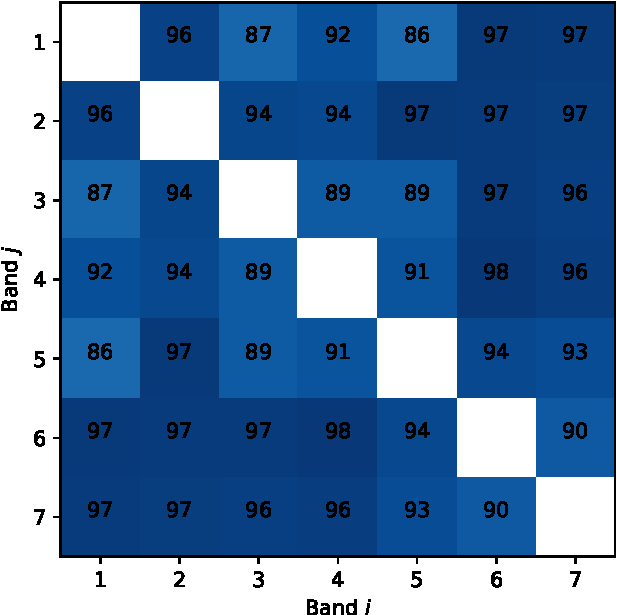
\includegraphics[width=0.9\linewidth]{sup-crop.pdf} 
    \caption{Logarithm applied} 
    \label{fig7:a} 
    %\vspace{4ex}
  \end{subfigure}%% 
  \begin{subfigure}[b]{0.49\linewidth}
    \centering
    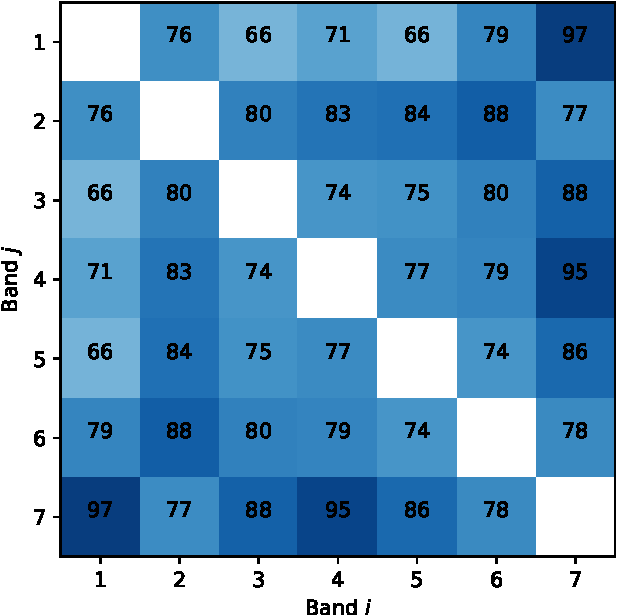
\includegraphics[width=0.9\textwidth]{un-crop.pdf} 
    \caption{Binary segmented image} 
    \label{fig7:b} 
    %\vspace{13ex}
    \end{subfigure} 
  \begin{subfigure}[b]{0.49\linewidth}
    \centering
    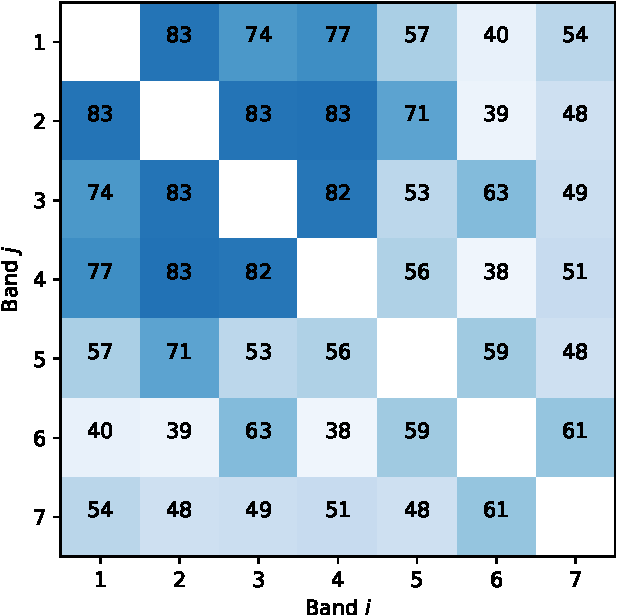
\includegraphics[width=0.9\textwidth]{kmeans-crop.pdf} 
    \caption{Hough Transform} 
    \label{fig7:c} 
  \end{subfigure}%%
  \begin{subfigure}[b]{0.49\linewidth}
    \centering
    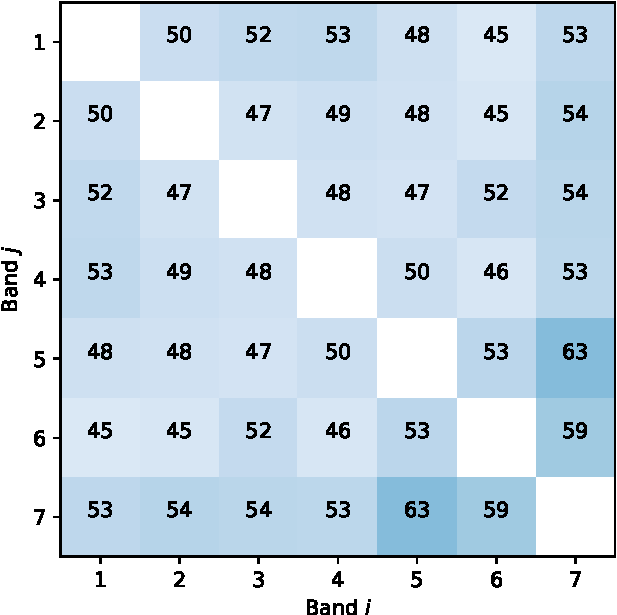
\includegraphics[width=0.9\textwidth]{gmm-crop.pdf} 
    \caption{Segmented image} 
    \label{fig7:d} 
  \end{subfigure} 
  \caption{c}
  \label{fig7} 
\end{figure*}





\section{Conclusion}
\label{sec:ref}
We presented a label agnostic feature extraction comparison framework in this paper. We demonstrated its usefulness by employing it and a case study to compare two feature extraction methods,
namely FFT and PCA (we also found that the PCA approach outperformed the FFT approach).

%List and number all bibliographical references at the end of the paper.  The references can be numbered in alphabetic order or in order of appearance in the document.  When referring to them in the text, type the corresponding reference number in square brackets as shown at the end of this sentence \cite{C2}.

% References should be produced using the bibtex program from suitable
% BiBTeX files (here: strings, refs, manuals). The IEEEbib.bst bibliography
% style file from IEEE produces unsorted bibliography list.
% -------------------------------------------------------------------------
\bibliographystyle{IEEEbib}
\bibliography{strings,refs}

\end{document}
